\section{Evaluation}
\label{lance-sec-evaluation}

\begin{figure}[t]
\begin{center}
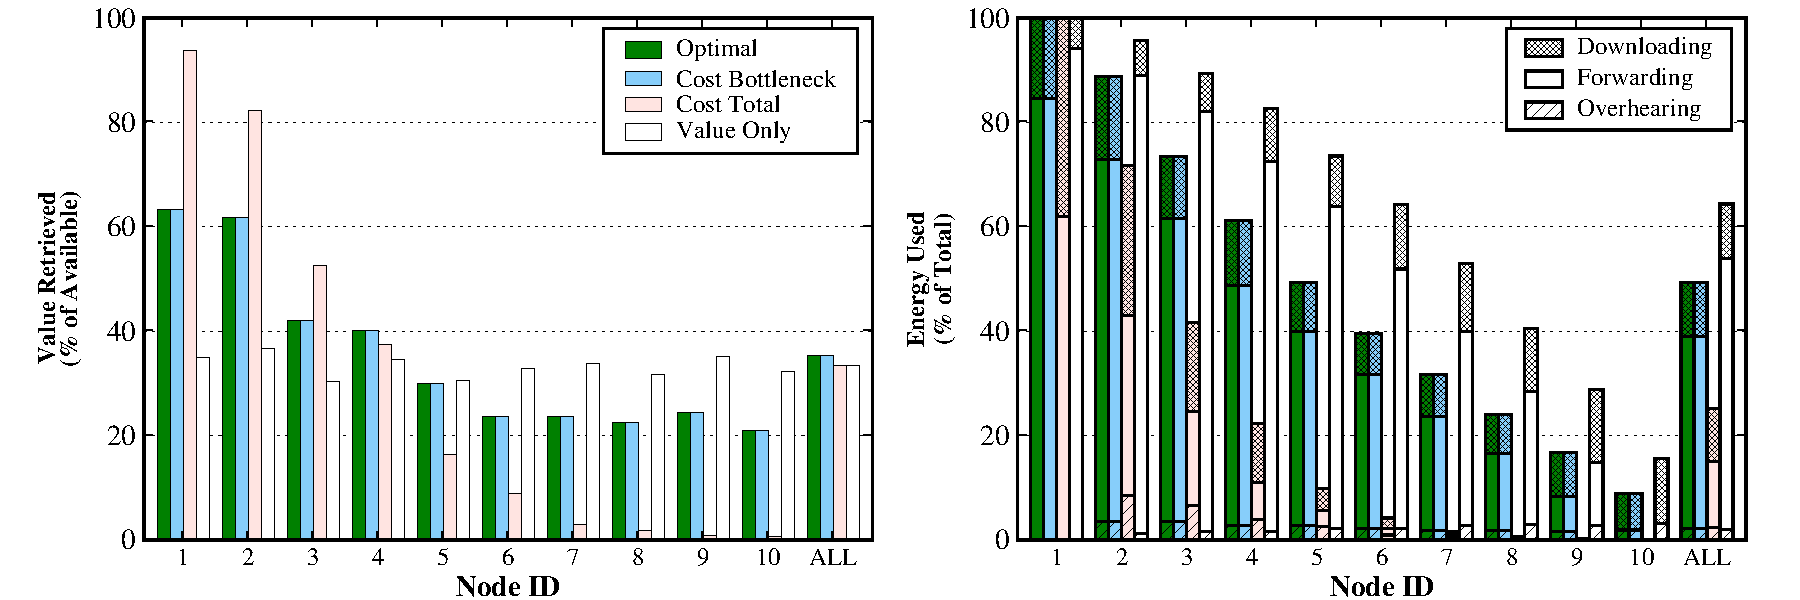
\includegraphics[width=1.0\hsize]{./4-lance/figs/linear.pdf}
\end{center}

\caption{\textbf{Per-node distribution of ADU value and energy usage for the
linear simulation experiment.} The top graph shows the amount of data value
downloaded from each node, while the bottom graph breaks down the amount of
energy used by each node into the downloading, routing and overhearing
components. Node~1 is closest to the base station.}

\label{lance-fig-linear}
\end{figure}

\begin{figure}[t]
\begin{center}
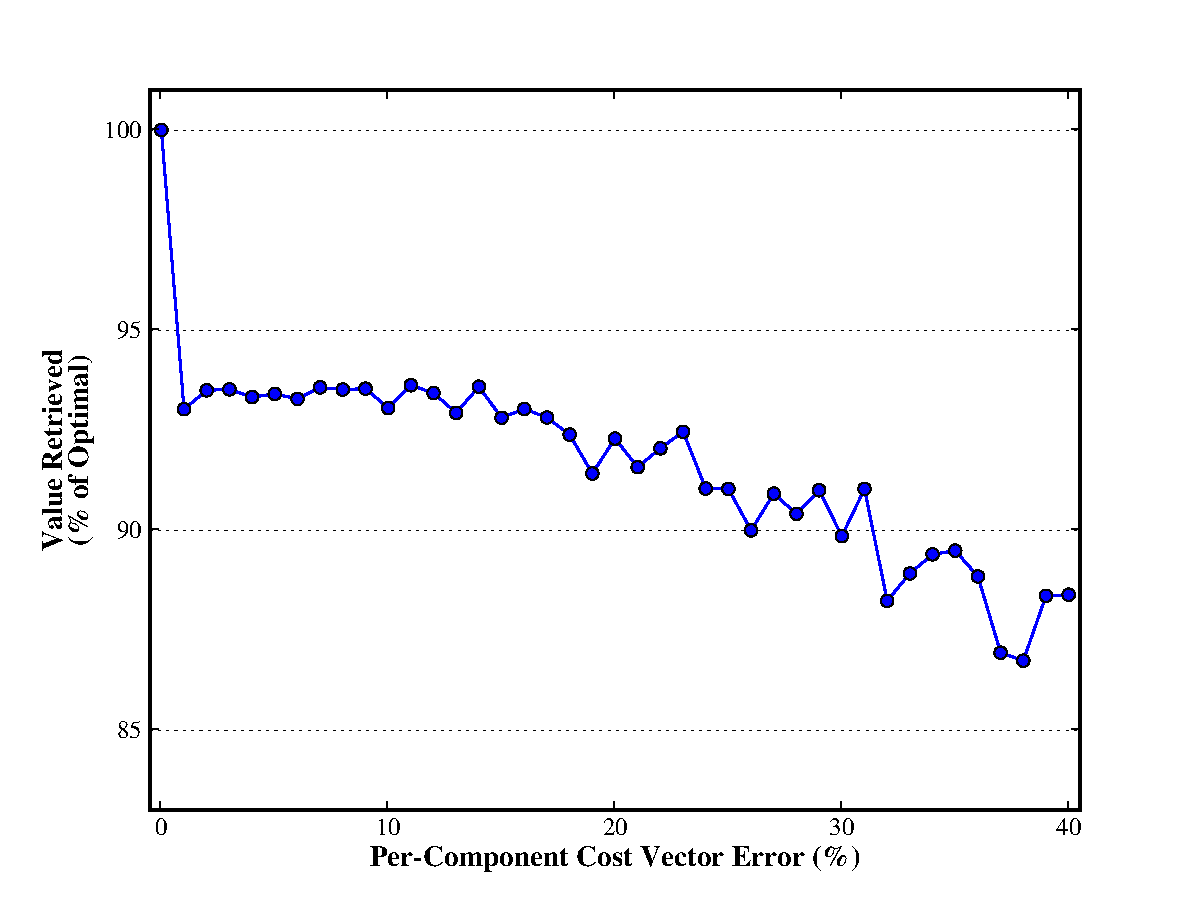
\includegraphics[width=1.0\hsize]{./4-lance/figs/error.pdf}
\end{center}

\caption{\textbf{Effect of cost vector error on optimality.} The optimization
process is guided by the cost vectors, but predicting the energy cost of
operations before they are performed can be difficult. Here we show the
impact of introducing a degree of error into the cost vectors used by the
optimizer. As can be seen, we can tolerate a relatively high degree of error,
as long as the shape of the cost vector does not change.}

\label{lance-fig-error}
\end{figure}

This section presents a careful evaluation of Lance conducted along several
lines. Using a high-level system simulator and synthetic data sets, we
evaluate the three scoring functions described in
Section~\ref{lance-subsec-optimizer}. We motivate the use of the
\textit{cost-bottleneck} scoring function and demonstrate that it performs
better than simpler alternatives. Next, we look at the effect of varying
parameters such as download bandwidth and network lifetime, as well as the
impact of errors in the cost vectors. We also present results from
experiments run on a 50-node sensor network testbed using realistic data
sets.

\subsection{Metrics and Methodology}

\begin{figure}[t]
\begin{center}
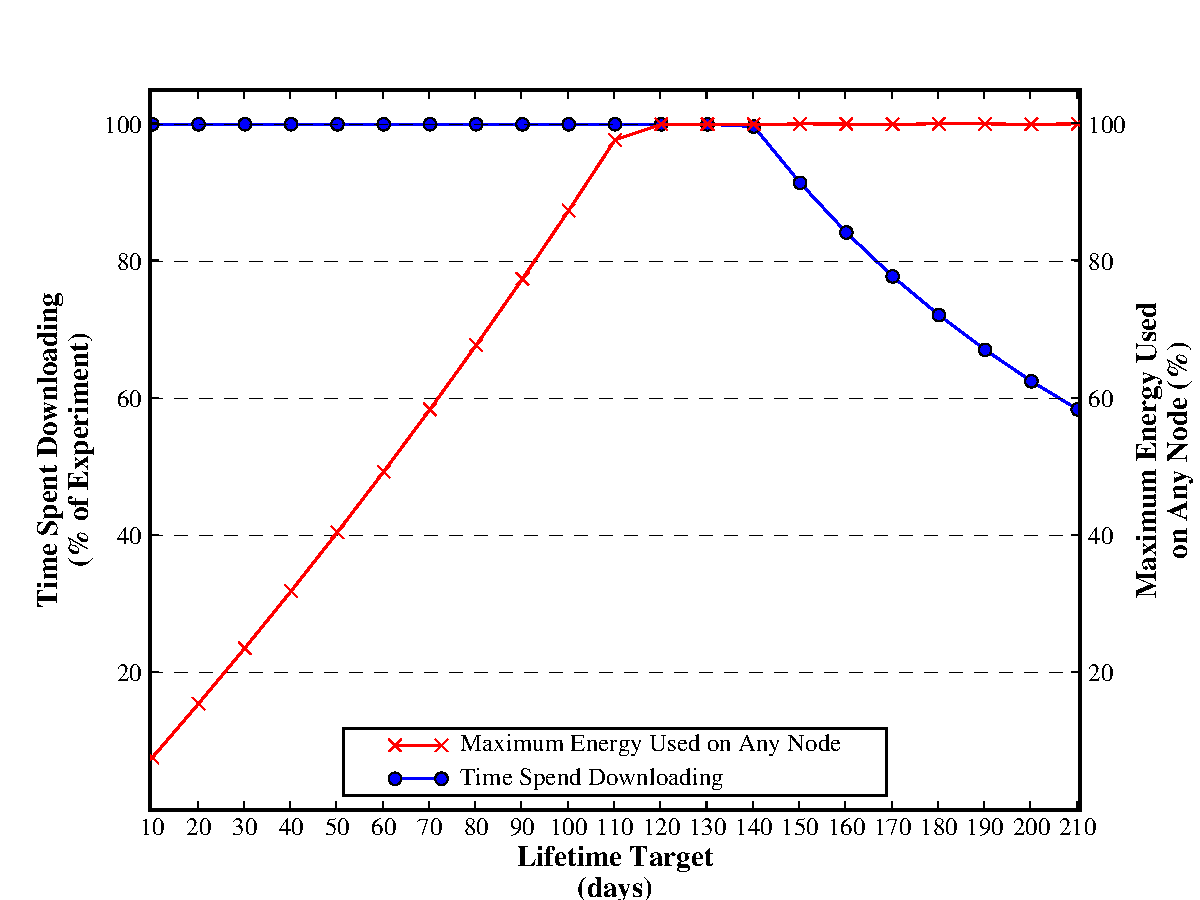
\includegraphics[width=1.0\hsize]{./4-lance/figs/crossover.pdf}
\end{center}

\caption{\textbf{Crossover between bandwidth and energy constraint dominance
as lifetime is varied.} This graph shows the transition between bandwidth and
energy constrained regions for an optimal system. The right axis shows the
percent of energy consumed by the most highly-drained node, and the left axis
shows the amount of time spent downloading.}

\label{lance-fig-crossover}
\end{figure}

As stated in Section~\ref{lance-sec-problem-definition}, the high-level goal
of Lance is to download a set of ADUs maximizing the total value subject to
energy and bandwidth constraints. The \textit{optimal} solution is defined as
the solution to the multidimensional knapsack problem, which yields a set of
downloaded ADUs $\mathcal{O} = \{a_1, a_2, ... a_n\}$ that maximize data
value subject to bandwidth and energy constraints. The total data value of
the optimal solution $\hat{v}(\mathcal{O}) = \sum_{a_i \in \mathcal{O}} v_i$.
Recall that computing the optimal solution requires \textit{a priori}
knowledge of all of the ADU values sampled by the network over time. We
define \textit{optimality} as the fraction of the data value downloaded by
Lance compared to the optimal solution. That is, given a set of downloaded
ADUs $\mathcal{L}$ with total data value $v(\mathcal{L})$, we define
optimality as $v(\mathcal{L}) / \hat{v}(\mathcal{O})$.

We begin by presenting results based on a realistic system simulator that
allows us to quickly vary parameters such as ADU data value distribution,
network topologies, download speeds, energy costs, and target lifetimes. We
also present results from Lance running on MoteLab~\cite{motelab}, a sensor
network testbed deployed over 3~floors of the Harvard EECS building. Our
simulation experiments use a 10-node linear topology as well as a 25-node
realistic tree topology shown in Figure~\ref{lance-fig-topology}(a).
Both topologies use per-node ADU download speeds based on empirical
measurements taken using the testbed. In our experiments, the ADU size is
36~KB and each node samples one ADU every 60~s (or 600~Bps of data).

We draw ADU values from several distributions in an attempt to understand
Lance's behavior as the properties of the sampled data change. Three value
distributions are used: uniform random, exponentially distributed, and Zipf
with exponent $\alpha = 1$. We also make use of an ADU value distribution
based on a 6~hour seismic signal collected at Reventador Volcano, Ecuador in
2005. Except where stated, no policy modules were used. In order to compute
optimal solutions, we frame the problem as a multi-dimensional knapsack
problem as previously described and solve the resulting instance using
\texttt{lpsolve}.

The energy costs for various operations are modeled as follows. The
background current drain of each node is set to 2~mA, based on empirical
measurements of a TMote~Sky sensor node performing high-data-rate sampling
and storing to flash. We also measured the current consumption to download an
ADU from a sensor node, and derived the energy costs for downloading ($E_d =
17.6$~mA/s), routing ($E_r = 16.9$~mA/s), and overhearing ($E_o = 2$~mA/s).
Our experiments assume that each node can only overhear its parent in the
routing tree; developing more detailed overhearing models is the subject of
future work. Computing the components of the cost vector for a particular ADU
is done by multiplying the current consumption by the ADU download time for
each node either downloading, routing, or overhearing the transmission.

\subsection{Effectiveness of Scoring Functions}
\label{lance-sec-eval-heuristics}

\begin{figure}[t]
\begin{center}
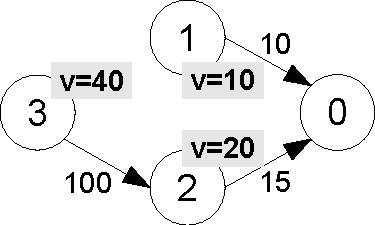
\includegraphics[width=1.0\hsize]{./4-lance/figs/motivationexample.pdf}
\end{center}

\caption{\textbf{Example simple download problem.}}

\label{lance-fig-simple}
\end{figure}

\begin{table}[t]
\begin{center}
\begin{tabular}{|l|l|ccc|}
\hline
& & \multicolumn{3}{|c|}{Scoring Functions} \\ \hline
& & Value & Cost & Cost \\
Distribution & Lifetime & Only & Total & Bottleneck \\ \hline
\multirow{3}{*}{Uniform} & 4 months & 62.4\% & 90.5\% & \textbf{93.2\%} \\
& 11 months & 43.4\% & 68.0\% & \textbf{96.9\%} \\
& 18 months & 44.6\% & 49.0\% & \textbf{90.0\%} \\ \hline
\multirow{3}{*}{Exponential} & 4 months & 83.9\% & 85.1\% & \textbf{88.0\%}
\\
& 11 months & 70.4\% & 82.0\% & \textbf{93.0\%} \\
& 18 months & 67.2\% & 72.8\% & \textbf{91.2\%} \\ \hline
\multirow{3}{*}{Zipfian} & 4 months & 84.7\% & \textbf{91.4\%} & 87.1\% \\
& 11 months & 63.8\% & 91.1\% & \textbf{96.2\%} \\
& 18 months & 53.1\% & 86.9\% & \textbf{93.8\%} \\ \hline
\end{tabular}
\end{center}

\caption{\textbf{Optimality of different scoring functions.} This table
summarizes simulation results evaluating the three different scoring
functions. Results are shown for several different lifetime targets and value
distributions. \textit{cost-bottleneck} out-performs the others in almost all
cases.}

\label{lance-fig-table}
\end{table}

We begin by evaluating the three scoring functions described
Section~\ref{lance-subsec-optimizer}. We want to see which is the most able
to approximate the optimal solution across a range of target lifetimes and
ADU distributions. As discussed earlier we expected the \textit{value-only}
scoring function, without considering the energy or bandwidth overhead of
downloading each ADU, to consume more energy downloading high-valued ADUs
when it could have increased the total data value by downloading several
slightly less-highly valued ADUs with lower costs. The \textit{cost-total}
scoring function incorporates a notion of cost, but will tend to favor nodes
closer to the base station at the expense of high-valued ADUs that are more
routing hops away. The \textit{cost-bottleneck} scoring function should
strike a balance between the two, since it considers only the most
significant cost vector component.

To develop intuition, consider the simple download problem shown in
Figure~\ref{lance-fig-simple}. The figure shows the network topology with the
energy required to reliably use each link labeled. Note that since we assume
that node radios are left on throughout the transfer the cost to route data
towards the sink is driven by the worst link along the path. links. So
Nodes~2 and 1 in the figure shown will have a cost of 100~units to route each
packet for Node~3 due to the poor link between Nodes~2 and 3. Three ADUs are
available in the network, one at each of nodes 1, 2, and 3, and the values of
each are labeled. Also assume that Nodes 1, 2 and 3 have 300, 600 and 2,000
units of available energy, respectively.

The question is: given the battery states, download costs, and values of each
ADU, which ADU should Lance download? To summarize the three ADUs available:

\begin{itemize}

\item \textbf{$ADU_1$}: located at Node~1 with value $v_1 = 10$ and cost vector
$\bar{c}_1 = \left[10, 0, 0\right]$. Note we are not considering the cost at the base
station, which we assume to be powered.
\vspace*{-0.1in}
\item \textbf{$ADU_2$}: located at Node~2 with value $v_2 = 20$ and cost vector
$\bar{c}_2 = \left[15, 15, 0\right]$.
\vspace*{-0.1in}
\item \textbf{$ADU_3$}: located at Node~3 with value $v_3 = 40$ and cost vector
$\bar{c}_3 = \left[100, 100, 100\right]$.

\end{itemize}


For this example, the three scoring functions make three different choices:

\begin{itemize}

\item \textbf{\textit{value-only}} will choose the ADU with the highest
value, $ADU_3$, regardless of the energy impact on the network.

\item \textbf{\textit{cost-total}} will compute the total cost of each ADU
and use that to weight the ADU's value. For this set of ADUs, $ADU_1$ has the
best ratio of value to total cost of the three choices: $0.1$, $0.066$ and
$0.013$ respectively.

\item \textbf{\textit{cost-bottleneck}} will first compute the bottleneck
node for each ADU by determining which node will be the most impacted by
downloading it. In this case, Node~1 is the bottleneck node for all three
ADUs, since it must devote 3.3\% of its remaining energy to $ADU_1$ (versus
0\% for Nodes~2 and 3), 5.0\% to $ADU_2$ (versus 2.5\% for Node~2 and 0\% for
Node~3), and 33\% to $ADU_3$ (versus 16\% for Node~2 and 5\% for Node~3).

\hspace{0.25in} Identifying the bottleneck cost causes
\textit{cost-bottleneck} to choose $ADU_2$, which has the best ratio of value
to  bottleneck cost (or cost to Node~1 in this case): $0.13$ versus $0.1$ for
$ADU_1$ and $0.04$ for $ADU_3$.

\end{itemize}

To convince ourselves that the \textit{cost-bottleneck} scoring function has
made the correct choice for this simple example, imagine that we can
repeatedly download ADUs with these values from each node in the network
until nodes run out of energy. We can download 30 copies of $ADU_1$ for a
total value of 300, 20 copies of $ADU_2$ for a total value of 400, or 3
copies of $ADU_3$ for a total value of 120. $ADU_2$ is the correct choice.

In many cases the node connecting the network to the powered sink quickly
becomes the bottleneck node, since all network traffic must be routed through
it. Figure~\ref{lance-fig-linear} shows simulation results using the 10-node
linear topology with exponentially-distributed ADU values, and a target
lifetime of 3~months. Nodes are numbered in increasing distance from the base
station. The graph confirms the intuition behind the scoring function
behavior. \textit{value-only} downloads roughly equal value from each node,
but fails to match the optimal performance. \textit{cost-total} downloads
more data from nodes near the sink. \textit{cost-bottleneck} comes close to
matching the optimal solution, retrieving over 99\% of the value retrieved by
the optimal solution. The smooth fall-off in the amount of value downloaded
from each node is a result of the decaying transfer speeds as the protocol
must communicate with nodes deeper in the tree. Node~1 is always the
bottleneck node during this experiment.

\begin{figure}[t]
\begin{center}
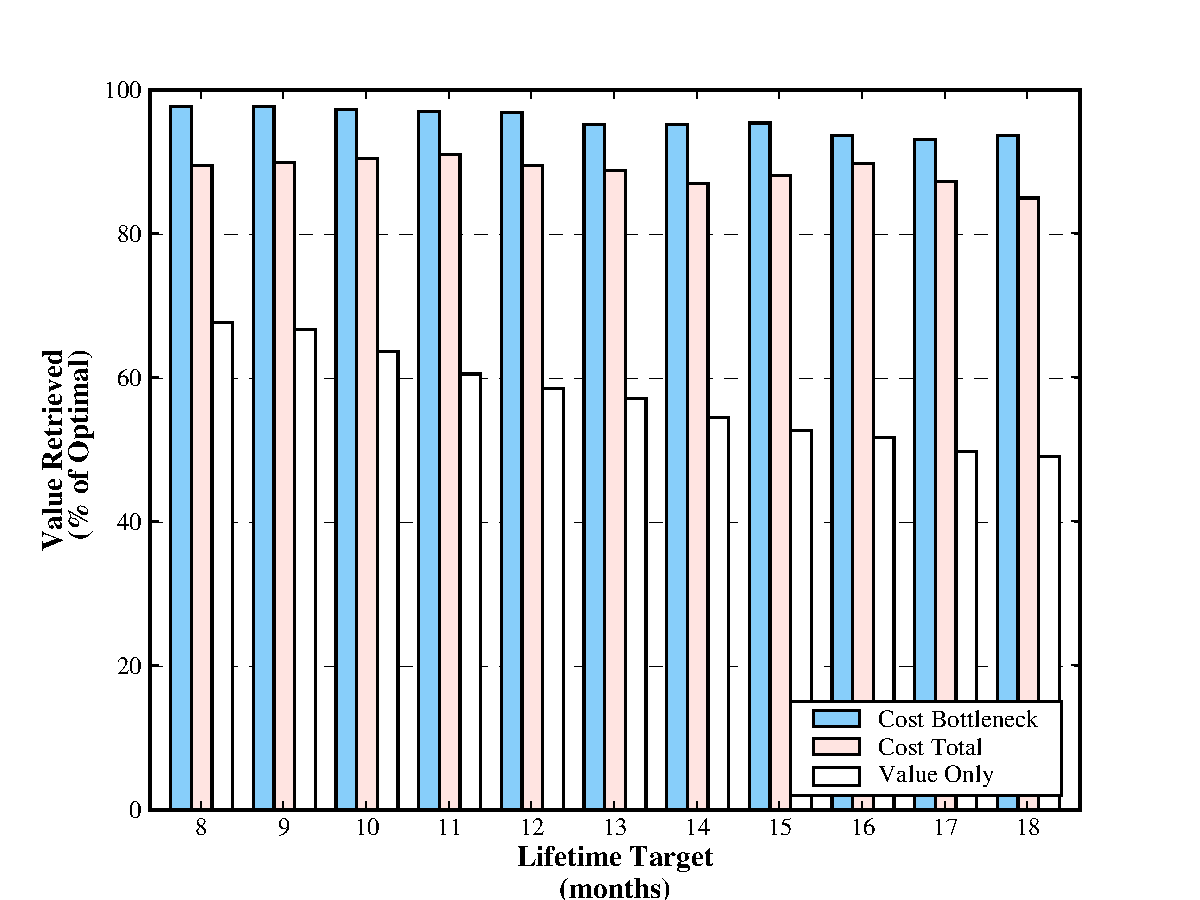
\includegraphics[width=1.0\hsize]{./4-lance/figs/zipfian.pdf}
\end{center}

\caption{\textbf{Scoring function performance on Zipfian distribution.} The
\textit{cost-bottleneck} scoring function outperforms the other two across a
range of lifetime targets.}

\label{lance-fig-zipfian}
\end{figure}

\begin{figure}[t]
\begin{center}
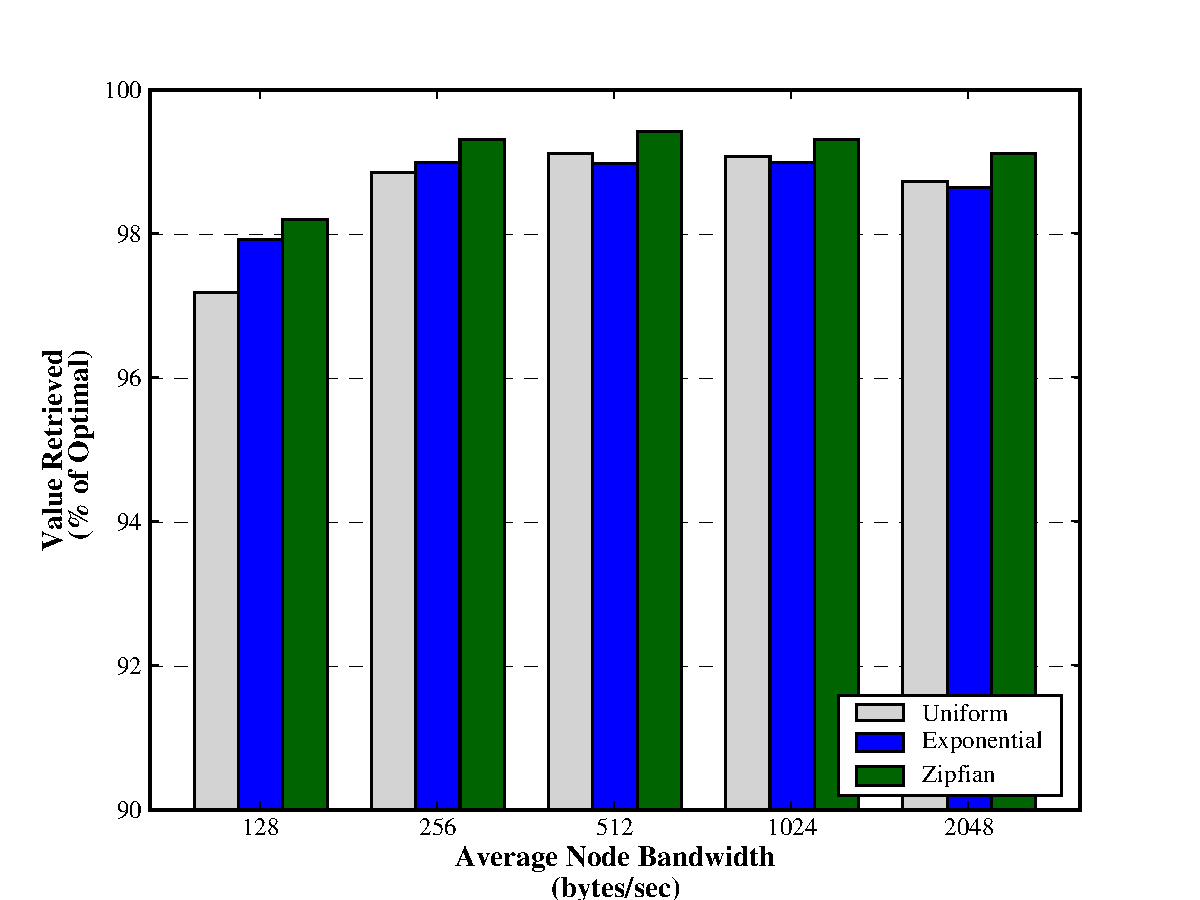
\includegraphics[width=1.0\hsize]{./4-lance/figs/speeds.pdf}
\end{center}

\caption{\textbf{Effect of varying download bandwidth.} Lance maintains a
high degree of optimality as the per-node download bandwidth is varied. Here
results are shown for the three synthetic distributions across a 25~node tree
topology and the \textit{cost-bottleneck} scoring function. Note that the
$y$-axis starts at 90\%.}

\label{lance-fig-speeds}
\end{figure}


Table~\ref{lance-fig-table} summarizes simulation results from a variety of
different lifetimes and value distributions, run on the 25-node tree
topology. The table shows that the \textit{cost-bottleneck} scoring function
outperforms the other two in most cases, with optimality values between
87.1\% and 96.9\%. The one exception is the 4-month Zipfian data set, where
\textit{cost-total} slightly outperforms \textit{cost-bottleneck}.
Figure~\ref{lance-fig-zipfian} shows the effect of varying the network's
target lifetime, using the 25-node tree topology and a Zipfian data value
distribution. As the figure shows, the \textit{cost-bottleneck} scoring
function maintains a high degree of optimality as the network bandwidth
changes.

\vfill\eject

To illustrate the effect of varying lifetime targets in more detail,
Figure~\ref{lance-fig-crossover} shows how the optimal solution transitions
between bandwidth-dominant and energy-dominant constraints as the target
lifetime increases. At low lifetime targets, the system is bandwidth
constrained and cannot download data fast enough to exhaust the nodes'
batteries. At high lifetime targets, the system is energy constrained and
cannot download continuously without exhausting the nodes' batteries.

\subsection{Bandwidth Adaptation}
\label{lance-sec-eval-params}

Next, we evaluate the impact of varying the download bandwidth in
Figure~\ref{lance-fig-speeds}, using the 25-node tree topology and the
\textit{cost-bottleneck} scoring function. We vary the per-node download
bandwidth from 128~to~2048~Bps and peg the target lifetime at 8~months.
As the figure shows, Lance performs well across the range of bandwidths, with
optimality greater than 97\% in all cases.

\subsection{Effect of Cost Vector Error}

Our last simulation study evaluates the effect of introducing errors into
estimated download cost. This experiment uses the 25-node topology,
\textit{cost-bottleneck} scoring function, and an exponential data
distribution. As described in Section~\ref{lance-subsec-costestimation}
estimating the cost of performing different operations \textit{a priori} can
be difficult. As shown in Figure~\ref{lance-fig-error}, even a 40\% error in
each component of the cost vector $\bar{c}_i$ for a given ADU only degrades
optimality by approximately 15\%. We conclude that accurate estimations of
download costs are not strictly necessary to achieve good performance.

Note that \textit{cost-bottleneck} depends on the ability to correctly
identify the bottleneck node. This is critical as that is the node whose cost
will be used to weight the value. In general we cannot compute the cost
perfectly \textit{a priori}, as described above. If two nodes have similar
values of $B(a_i,n)$ during the calculation of the bottleneck score, it is
possible that, assuming some error in the cost vector $\bar{c}_i$, we will
identify the wrong bottleneck and weight the value incorrectly. If the errors
are evenly distributed then over time we expect these mistakes to even out.
However, if there is a persistent miscalculation affecting one or both of the
nodes then we may repeatedly identify the wrong node as the bottleneck,
reducing optimality.

\subsection{Testbed Experiments}
\label{lance-sec-eval-policies}

\begin{figure}[t]
\begin{center}
\begin{tabular}{cc}
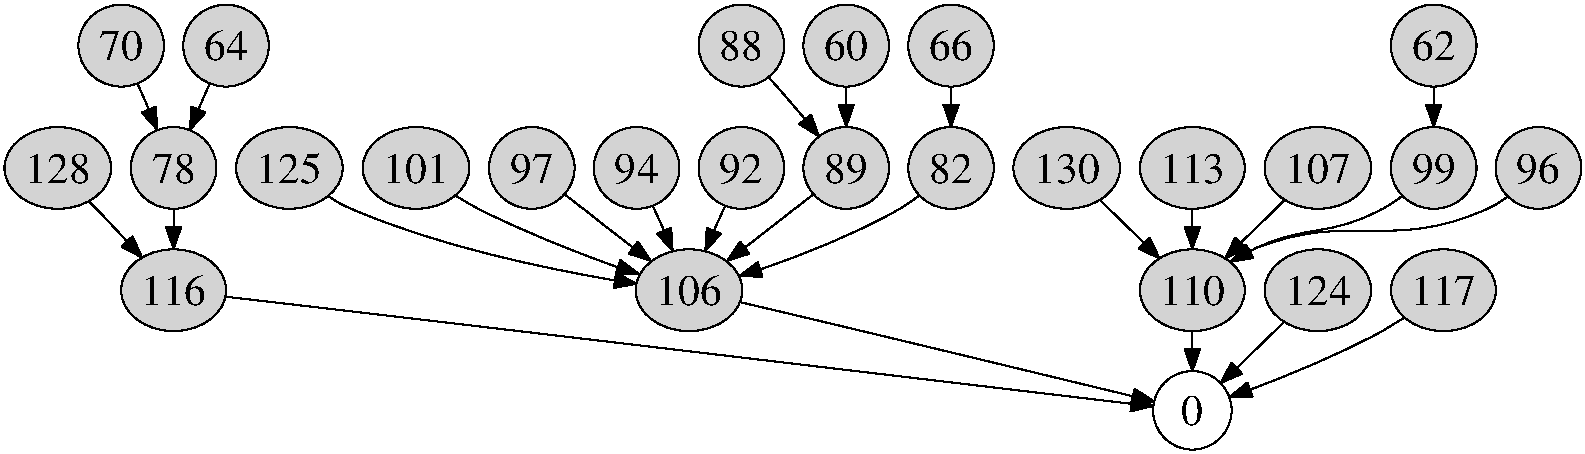
\includegraphics[width=0.45\hsize]{./4-lance/figs/topology25.pdf} &
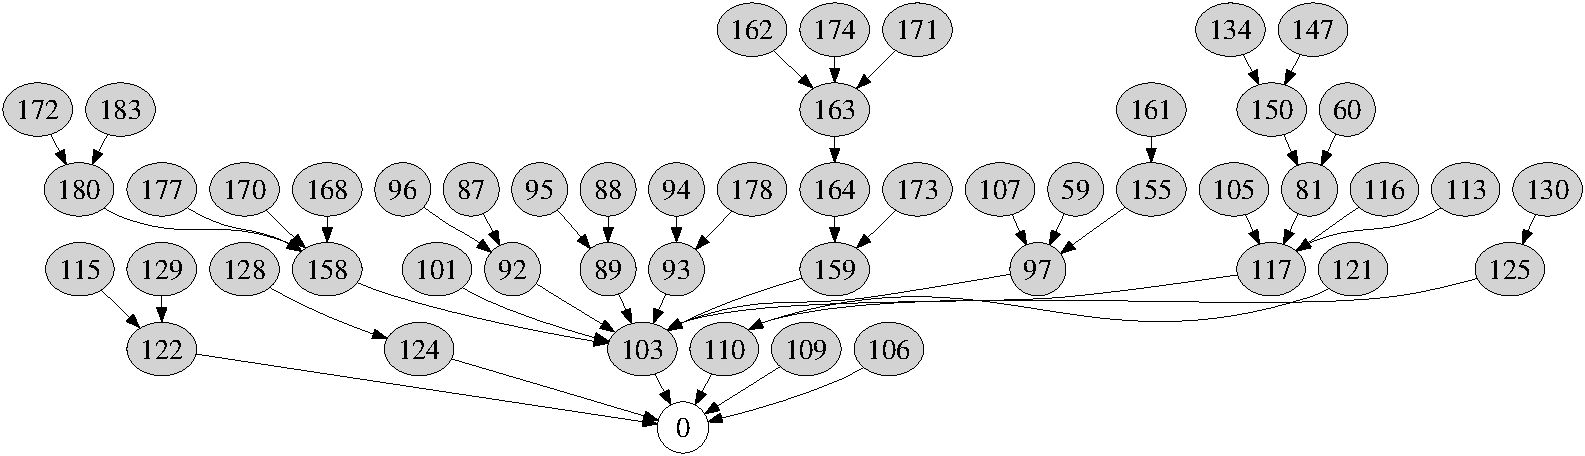
\includegraphics[width=0.45\hsize]{./4-lance/figs/topology50.pdf} \\
\textbf{(a)} &
\textbf{(b)} \\
\end{tabular}
\end{center}

\caption{\textbf{Topologies for testbed experiments.} This graph shows the 25
(a) and 50 (b) node topologies used for our testbed experiments.}

\label{lance-fig-topology}
\end{figure}

\begin{figure}[t]
\begin{center}
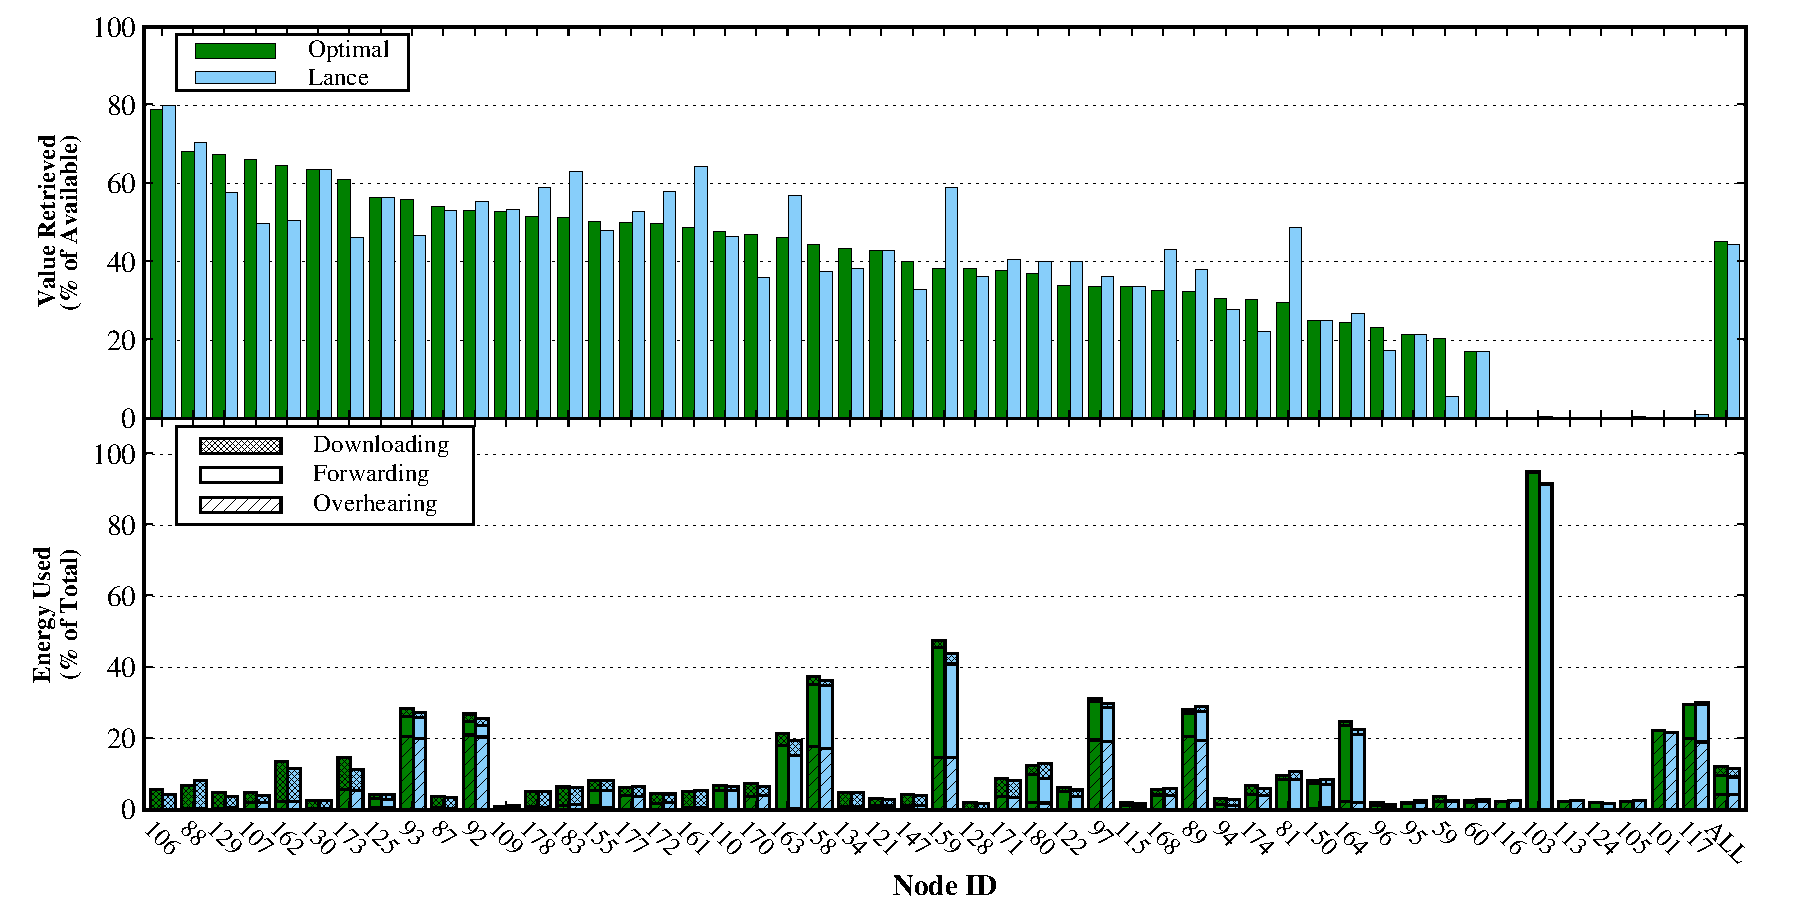
\includegraphics[width=1.0\hsize]{./4-lance/figs/big.pdf}
\end{center}

\caption{\textbf{Optimality and energy use in the 50-node testbed
experiment.} Lance achieved near-optimal performance during this 8-hour
testbed experiment, retrieving 98\% of the value obtained by the offline
optimal algorithm.}

\label{lance-fig-big}
\end{figure}

In this section, we present results from the Lance system running on the
MoteLab testbed, in 25-node and 50-node configurations shown in
Figure~\ref{lance-fig-topology}. These experiments stress the system in a
realistic setting subject to radio interference and congestion, exercising
the multihop routing protocol, Fetch reliable data-collection protocol, and
ADU summary traffic generated by the nodes. For these experiments, we
injected artificial ADU values directly into each node rather than relying on
the nodes sampling real sensor data; this approach allows us to perform
repeatable experiments that explore a wider range of ADU value distributions.
We use the \textit{cost-bottleneck} scoring function.

Figure~\ref{lance-fig-big} shows the results of a 50-node testbed experiment
using a Zipfian data distribution and a target lifetime of 6~months. The
upper portion of the figure shows the amount of data value obtained by Lance
from each node, compared to the optimal solution (which was computed
offline). Nodes are sorted by decreasing optimal value. As the figure shows,
Lance achieves close to the optimal solution, with an optimality of 98\%
overall. In some cases, Lance incorrectly downloads more data from some nodes
and less data from others; this is due to the inherent limitations of an
online solution that cannot foresee future ADU values. The lower portion of
the figure shows the energy breakdown for each node with downloading,
forwarding, and overhearing costs shown. Some nodes consume more than others
because of their location in the routing tree. For example, node~103 uses a
great deal of energy for routing packets as it is one hop from the base
station, although no ADUs are ever downloaded from that node.

\begin{figure}[t!]
\begin{center}
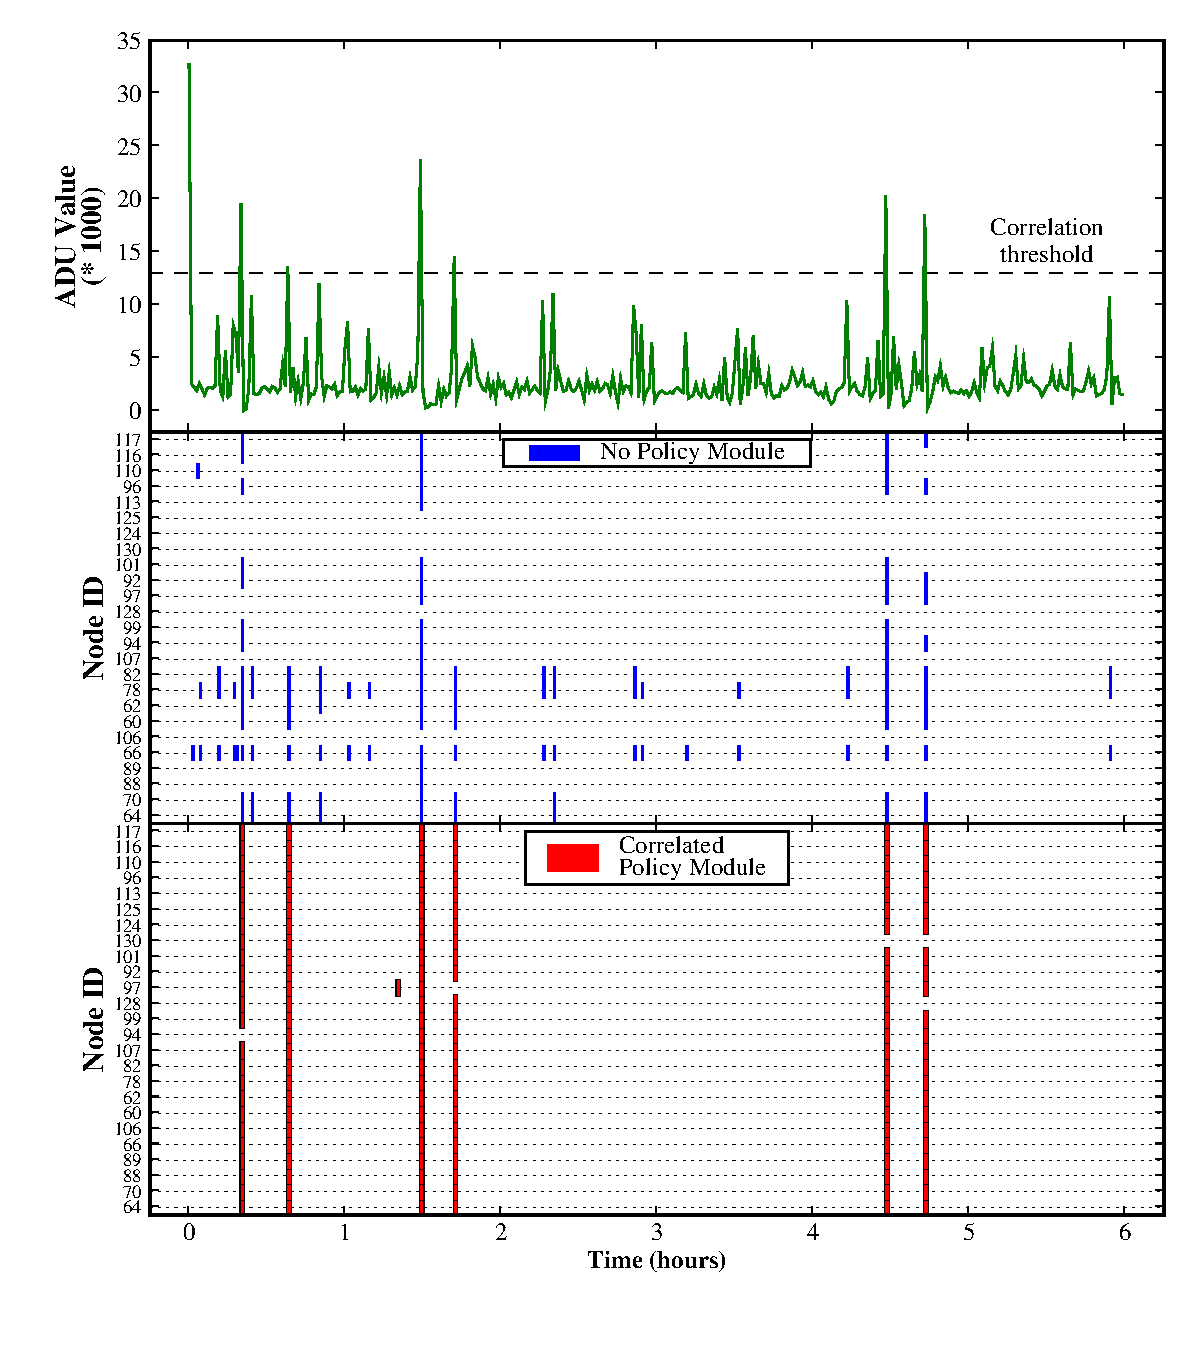
\includegraphics[width=0.7\hsize]{./4-lance/figs/fill.pdf}
\end{center}

\caption{\textbf{Usage of policy modules to affect download distribution.}
Here we illustrate the use of policy modules in the context of the
volcano-monitoring application. The graph compares the download behavior of
the system with and without the policy module chain described in
Section~\ref{lance-sec-ewma-deployment}, which assign greater values to ADUs
corresponding to correlated seismic activity. The graph is colored at a
particular timestamp and node ID if we downloaded that signal from that node.
The top graph shows the ADU values over time, with the threshold for the
\texttt{filter} component of the policy module chain indicated.}

\label{lance-fig-fill}
\end{figure}

Finally, we demonstrate the use of Lance's policy modules. For this
experiment, we use a distribution of ADU data values based on a 6-hour
seismic trace collected at Reventador Volcano, Ecuador in
2005. The raw seismic data is divided into ADUs of 36
KB and ADU values $v_i$ are assigned by computing the ratio of two
EWMA~filters on the data; this assigns greater value to ADUs that contain
earthquakes, as described in Section~\ref{lance-sec-ewma-deployment}. For
each node in the 25-node topology, the ADU values from the seismic trace are
attenuated based on a hypothetical signal source and assigned to each of the
25-nodes based on their location with respect to the signal source. We then
enable a policy module chain, as described in
Section~\ref{lance-sec-policies}, that assigns higher priority to ADUs that
correspond to correlated seismic activity across the network.

Figure~\ref{lance-fig-fill} shows the result of this experiment running on
the MoteLab testbed. The upper portion of the figure shows the ADU values
over time; the middle portion, the set of ADUs downloaded by the system with
no policy modules in use; and the lower portion, the ADUs downloaded with the
policy module chain in use. As the figure shows, the policy modules cause the
network to prefer correlated seismic events and download an ADU from all
nodes in the network when such an event is detected. Gaps in the set of ADUs
downloaded are due to download timeouts. In one case, a single ADU is
downloaded spuriously due to an incorrect value being reported by that node
to the base station. This use of policy modules shows the drastic change in
the system behavior that is affected without programming the sensor nodes
themselves.
